\section{Bridge}

\begin{figure}[htb]
	\caption{\label{bridge_struct}Estrutura do Bridge}
	\begin{center}
	    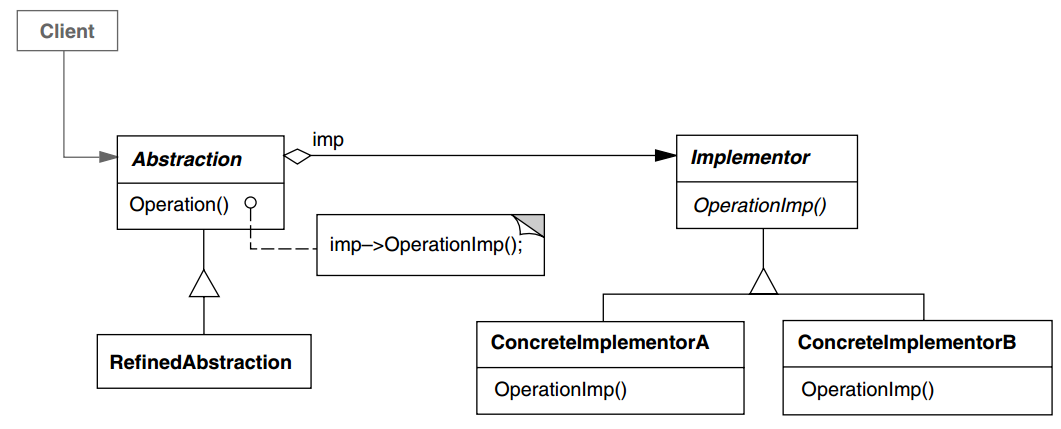
\includegraphics[scale=0.4]{5_padroes-contexto-funcional/5.2_estruturais/5.2.2_bridge/diagram.png}
	\end{center}
\end{figure}

\subsection*{Exemplo Orientado a Objetos}

\begin{figure}[htb]
	\caption{\label{bridge_exemplo}Exemplo de Bridge}
	\begin{center}
	    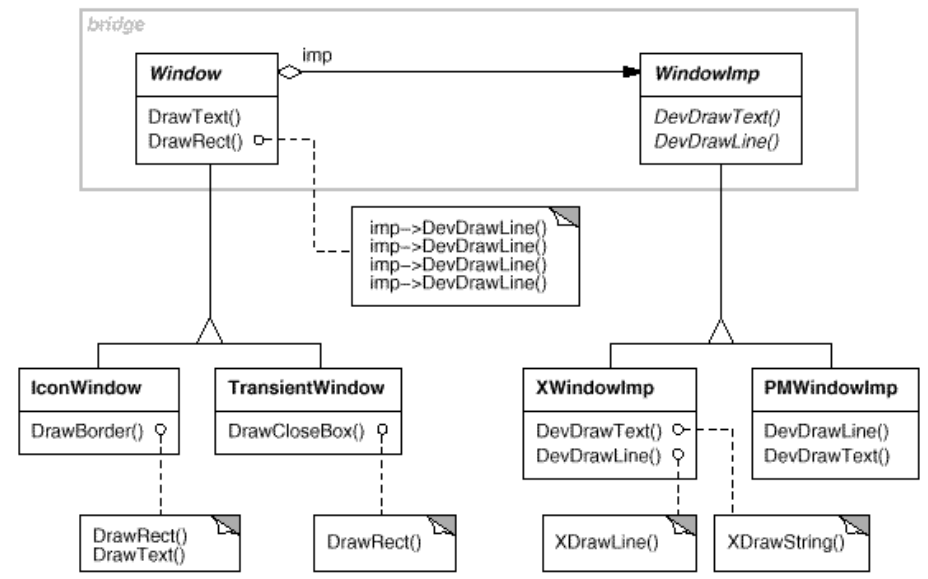
\includegraphics[scale=0.45]{5_padroes-contexto-funcional/5.2_estruturais/5.2.2_bridge/exemplo_bridge.png}
	\end{center}
\end{figure}

\begin{lstlisting}[caption={Bridge Orientado a Objetos},label=oobridge]

abstract class Window{
	var imp : WindowImp;

	def DrawText();
	def DrawRect();
}

class WindowImp(){
	def DevDrawText();
	def DevDrawLine();
}

class IconWindow() extends Window {
	def DrawBorder() {
		DrawRect();
		DrawText();
	}
}

class TransientWindow() extends Window {
	def DrawCloseBox() {
		DrawRect();
	}
}

class XWindowImp() extends WindowImp {
	def DevDrawText() {
		XDrawString();
	}

	def DevDrawLine() {
		XDrawLine();
	}
}

class PMWindowImp() extends WindowImp {
	def DevDrawLine() {
		PMDrawLine();
	}

	def DevDrawText() {
		PMDrawString();
	}
}

\end{lstlisting}


\subsection*{Contexto Funcional}

\begin{lstlisting}[caption={Bridge Funcional},label=fpbridge]
    

    
\end{lstlisting}